\documentclass{article}
\usepackage[utf8]{inputenc}
\usepackage[margin=0.5in,includefoot]{geometry}
\usepackage[export]{adjustbox}

% Header and Footer Setup
\usepackage{fancyhdr}
\pagestyle{fancy}
\fancyhead{}
\fancyfoot{}
\fancyfoot[R]{\thepage}
\renewcommand{\headrulewidth}{0pt}
\renewcommand{\footrulewidth}{0pt}
%
%Graphics Setup
\usepackage{graphicx}
\usepackage{float}
\usepackage{subfig}


%list setup
\usepackage{amssymb}
\renewcommand{\labelitemi}{$\blacktriangleright$}
\renewcommand{\labelitemii}{$\bullet$}
\renewcommand{\labelitemiii}{$\circ$}

%Source Code setup
\usepackage{xcolor}
\usepackage{listings}

\definecolor{mGreen}{rgb}{0,0.6,0}
\definecolor{mGray}{rgb}{0.5,0.5,0.5}
\definecolor{mPurple}{rgb}{0.58,0,0.82}
\definecolor{backgroundColour}{rgb}{0.95,0.95,0.92}

\lstdefinestyle{CStyle}{
    backgroundcolor=\color{backgroundColour},   
    commentstyle=\color{mGreen},
    keywordstyle=\color{magenta},
    numberstyle=\tiny\color{mGray},
    stringstyle=\color{mPurple},
    basicstyle=\footnotesize,
    breakatwhitespace=false,         
    breaklines=true,                 
    captionpos=b,                    
    keepspaces=true,                 
    numbers=left,                    
    numbersep=5pt,                  
    showspaces=false,                
    showstringspaces=false,
    showtabs=false,                  
    tabsize=2,
    language=C
}
%
\begin{document}

\begin{titlepage}

	\begin{flushright}
	\textsc{\large May 03, 2021} \\
	\end{flushright}
	\begin{center}
	\Large{\bfseries Gebze Technical University \\ Computer Engineering \\ CSE344 - Spring 2021 \\ MIDTERM} \\
	\end{center}
	\topskip0pt
	\vspace*{\fill}
	\begin{center}
	\Large{\bfseries Nevzat Seferoglu \\ 171044024 }
	\end{center}
	\vspace*{\fill}
\end{titlepage}

\cleardoublepage
\section{Problem Definition}
The problem was applying classical \textbf{producer-consumer} pattern. There is a clinic. There are nurses to bring vaccines to clinic. There are vaccinators which vaccinates the citizens which are wating for to be vaccinated for certain amount of doses. The paradign was clear. Nurses correspond to producer, vaccinator correspond to consumer. Each citizen must be vaccinated at least one pair dose which means that vaccinating for two times (specified before).

\section{Solution}
I exploited certain type of structures in that project. These are \textbf{unnamed semaphores}, \textbf{shared memory}. Each nurses, vaccinators and citizens are actual processes and need to communicate each other for synchronization and also sharing some resource all together.

\subsection{Design and Solutions}
\subsubsection{Shared Memory and Buffer Structure}
Shared memory is a well-known structure for communication between processes. There are common resources in that sturucture and each has to be altered synchronously. In that moment, semaphores step in. Semaphores are our main gun for synchronization between processes. I used \textbf{unnamed semaphores} intentionally. Unnamed semaphores are either private, inherited through fork(), or are protected by access protections of the regular file where they are allocated and mapped.
\begin{lstlisting}[style=CStyle]
typedef struct Buffer {
    sig_atomic_t sigint;    /* Reaching signal notification among processes. */
    int totalAppliedDose;
    int deadCitizen;
    long currCitizen;
    int nurseTermination;
    long fNurse, fVaccinator, fCitizen;
    int firstDose;
    int secDose;
    int fd;
    sem_t empty;        /* Synchronization purpose. (Producer get locks) */
    sem_t full;         /* Synchronization purpose. (Consumer get locks) */
    sem_t m;            /* Shared memory protection. */
    sem_t mConsumer;    /* Protecting for not to be blocked while consuming */
    sem_t mCitizen;     /* Citizen information sharing with vaccinator */
    sem_t mSafe;        /* Citizen information sharing with vaccinator */
} Buffer;
\end{lstlisting}
Shared memory is diretly returned to that structure. Every single variable that is kept in this structure are being used somewhere in code by more than two unrelated or related processes. The design makes me more comfortable to reach out some resources while multiprocessing.
\subsubsection{Nurse Design (the Producer)}
Nurses bring the vaccines one by one from the clinic until the vaccines are over. We were taking doses from file and each nurse needs to reach file synchronously. For that purpose I use inherited file descriptor which is opened in parent process. Each nurse takes the vaccines by protecting with mutex, bring them to clinic. The file could also include newline character so I designed a structure that ignores unrelated character which is taken from file.
\begin{lstlisting}[style=CStyle]
if (gfile->isEof) {
    ++gbuffer->nurseTermination;
    if (gbuffer->nurseTermination == numOfNurses)
        fprintf(stdout, "Nurses have carried all vaccines to the buffer, terminating.\n");
    x_sem_post(&(gbuffer->m));
    x_sem_post(&(gbuffer->full));
    break;
}
if (gfile->c != '1' && gfile->c != '2') {
    x_sem_post(&(gbuffer->m));
    x_sem_post(&(gbuffer->empty));
    continue;
}
/* Taken does is recorded to shared memory to be used by vaccinator. */
if (gfile->c == '1') {
    ++(gbuffer->firstDose);
    fprintf(stdout, "Nurse %2d (pid=%ld) has brought "
    "vacinne 1: the clinic has %2d vaccine1 and %2d vacinne 2.\n",
    ((int)(((long)getpid())-(gbuffer->fNurse)+1)), (long)getpid(),
    gbuffer->firstDose, gbuffer->secDose);
}
else if (gfile->c == '2') {
    ++(gbuffer->secDose);
    fprintf(stdout, "Nurse %2d (pid=%ld) has brought "
    "vacinne 2: the clinic has %2d vaccine1 and %2d vacinne 2.\n",
    ((int)(((long)getpid())-(gbuffer->fNurse)+1)), (long)getpid(),
    gbuffer->firstDose, gbuffer->secDose);
}
\end{lstlisting}
Nurses are actual producer. So I exploited producer solution for that type.
\begin{lstlisting}[style=CStyle]
x_sem_wait(&(gbuffer->empty));
if (gbuffer->sigint == 1) {
    x_sem_post(&(gbuffer->empty));
    exit(EXIT_FAILURE);
}
x_sem_wait(&(gbuffer->m));
/* Nurse Operation */
x_sem_post(&(gbuffer->m));
x_sem_post(&(gbuffer->full));
\end{lstlisting}
\textbf{Tricky Fragment}\\
The tricky part for the nurse is designing a structure to be ignored unrelated file input (without ruining general semaphore mechanism). And also all nurses need to be exited when at least one nurse encountered with EOF.
\subsubsection{Vaccinator Design (the Consumer)}
Vaccinators are our main consumer. They do more than one job for vaccination. Their first job is vaccination, second job is inviting citizen to vaccinate. They consumes vaccines which are located in common buffer stucture and if there are enough doses for vaccination, they simple invite citizen by using semaphore by using contractual mechanism with citizen processes. Other than these.
\begin{lstlisting}[style=CStyle]
/* Guarded by other semaphore */
if (!isThereAnyDose()) {
    x_sem_post(&(gbuffer->m));
    x_sem_post(&(gbuffer->full));
    x_sem_post(&(gbuffer->full));
    x_sem_post(&(gbuffer->mConsumer));
    continue;
}
/* Guarded by other semaphore */
\end{lstlisting}
It is checking the dose amount. If the doses do not enough for vaccination. It will wait for existence of enough vaccines. And then call the citizen by using 2 semaphores. These two semaphores are assure that each citizen will take vaccines and record his id in shared buffer structure one by one without ruining each other.
\begin{lstlisting}[style=CStyle]
/* Guarded by other semaphore */
x_sem_wait(&(gbuffer->mCitizen));
x_sem_wait(&(gbuffer->mSafe));
--(gbuffer->firstDose);
--(gbuffer->secDose);
++appliedDoses;
++(gbuffer->totalAppliedDose);
fprintf(stdout, "Vaccinator %d (pid=%ld) is inviting citizen pid=%ld to the clinic\n",
    ((int)((long)getpid()-(gbuffer->fVaccinator)+1)),
    ((long)getpid()),
    (gbuffer->currCitizen));
x_sem_post(&(gbuffer->mSafe));
/* Guarded by other semaphore */
\end{lstlisting}
When vaccinator is ready, he waits (invitation) for a citizen (CPU choice) to vaccinate. Alter the some value in comman buffer. Citizens are also using these two semaphores to record their PID in an instant structure for giving them to vaccinator. Vaccinators are actual consumer. But while producer is producing an item. In this project, consumer needs to consume two items (if exists).
\begin{lstlisting}[style=CStyle]
/* Warning: This is not an actual code. It is just general overview of solution. */
x_sem_wait(&(gbuffer->mConsumer));
x_sem_wait(&(gbuffer->full));
x_sem_wait(&(gbuffer->full));
x_sem_wait(&(gbuffer->m));
/* Vaccinator Operation */
x_sem_post(&(gbuffer->m));
x_sem_post(&(gbuffer->empty));
x_sem_post(&(gbuffer->empty));
x_sem_post(&(gbuffer->mConsumer));
\end{lstlisting}
\textbf{Tricky Fragment}\\
The tricky part for the vaccinator is consuming two doses by waiting nurses in a synchronize way. I did not use extra semaphores for each dose. I needed to design a structure which consume doses while only these two doses exists for both type (1,2) at the same time at least one. Otherwise it needs to skip its own turn to be filled with that both doses (1,2). If all doses are applied to citizens it needs to be exited with precise message.
\begin{lstlisting}[style=CStyle]
if (gbuffer->totalAppliedDose == numOfCitizens*numOfDose) {
    fprintf(stdout, "Vaccinator %d (pid=%ld) vaccinated %d doses. ",
    ((int)((long)getpid()-(gbuffer->fVaccinator)+1)),
    ((long)getpid()),
    appliedDoses);
    x_sem_post(&(gbuffer->m));
    x_sem_post(&(gbuffer->full));
    x_sem_post(&(gbuffer->full));
    x_sem_post(&(gbuffer->mConsumer));
    break;
}
\end{lstlisting}
\subsubsection{Citizen Design (Intermediary Processes)}
Citizens are processes which are invited by vaccinators. In my design, they are constantly ready for to be vaccinated. If the vaccinator invite the citizen with certain semaphores, they have some kind of \textbf{protocol} which collaborate on not to be interleaved by another citizen and also by another vaccinator.\\\\
\textbf{The Protocol}\\
Actually, the citizen is trying to be vaccinated constantly but will not be vaccinated until the vaccinator is ready to vaccinate. By using that protocol, any others cannot attempt to be vaccinated by current processing vaccinator until he release protocol semaphores.\\\\
\textbf{Note:} This protocol causes an output might seen not as expected. CPU choices also affect output.\textbf{ But all citizens vaccinated by certain vaccinator and that vaccinator invites correct citizens with correct PID in correct time.}
\begin{lstlisting}[style=CStyle]
/* Warning: This is not an actual code. It is just general overview of solution. */
x_sem_wait(&(gbuffer->mSafe));
x_sem_post(&(gbuffer->mCitizen));
gbuffer->currCitizen = (long)getpid();
fprintf(stdout, "Citizen %d (pid=%ld) is vaccinated for the %dst time:"
" the clinic has %d vaccine1 and %d vaccine2\n",
((int)(((long)getpid())-(gbuffer->fCitizen)+1)),
(long)(getpid()),
(numOfDose-i+1),
gbuffer->firstDose,
gbuffer->secDose);
x_sem_post(&(gbuffer->mSafe));
\end{lstlisting}
Counting Vaccinated Citizen
\begin{lstlisting}[style=CStyle]
/* Warning: This is not an actual code. It is just general overview of solution. */
x_sem_wait(&(gbuffer->mSafe));
++(gbuffer->deadCitizen);
if (gbuffer->deadCitizen == numOfCitizens) {
    fprintf(stdout, "All citizens have been vaccinated.\n");
}
else {
    fprintf(stdout, "citizen is leaving."
    " Remaining citizens to vaccinate: %d\n",(numOfCitizens-(gbuffer->deadCitizen)));
}
x_sem_post(&(gbuffer->mSafe));
\end{lstlisting}
\subsubsection{CTRL+C Handling}
In parent, there is an handler for entire program. I also put variable to detect SIGINT across processes that are member of shared memory. When one process encountered with SIGINT, any other processes are being informed atomically. They make their own clean up then exited immediately to parent process.
\begin{lstlisting}[style=CStyle]
/* Warning: This is not an actual code. It is just general overview of solution. */
void handler_SIGINT() {
    /* Detection */
    gbuffer->sigint = 1;
}
memset(&sa_SIGINT, 0, sizeof(sa_SIGINT));
sa_SIGINT.sa_handler = handler_SIGINT;
x_sigaction(SIGINT, &sa_SIGINT, NULL);

/* Example escaping from vaccinator */
if (gbuffer->sigint == 1) {
    x_sem_post(&(gbuffer->full));
    x_sem_post(&(gbuffer->full));
    x_sem_post(&(gbuffer->mConsumer));
    exit(EXIT_FAILURE);
}
\end{lstlisting}
\section{Which requirements I achieved ?}
I tested my project with several scripts. It works properly.
\begin{figure}[H]
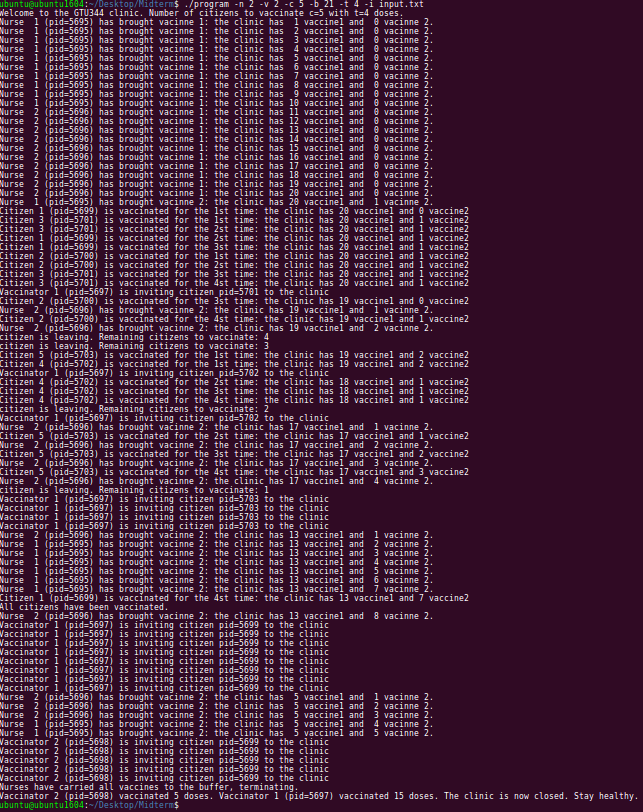
\includegraphics[width=1\textwidth, left]{output.png}
\caption[Optional caption]{}
\label{}
\end{figure}                    
\end{document}